\documentclass[]{article}
\usepackage{lmodern}
\usepackage{amssymb,amsmath}
\usepackage{ifxetex,ifluatex}
\usepackage{fixltx2e} % provides \textsubscript
\ifnum 0\ifxetex 1\fi\ifluatex 1\fi=0 % if pdftex
  \usepackage[T1]{fontenc}
  \usepackage[utf8]{inputenc}
\else % if luatex or xelatex
  \ifxetex
    \usepackage{mathspec}
  \else
    \usepackage{fontspec}
  \fi
  \defaultfontfeatures{Ligatures=TeX,Scale=MatchLowercase}
\fi
% use upquote if available, for straight quotes in verbatim environments
\IfFileExists{upquote.sty}{\usepackage{upquote}}{}
% use microtype if available
\IfFileExists{microtype.sty}{%
\usepackage{microtype}
\UseMicrotypeSet[protrusion]{basicmath} % disable protrusion for tt fonts
}{}
\usepackage[margin=1in]{geometry}
\usepackage{hyperref}
\hypersetup{unicode=true,
            pdftitle={DATA 606 - Homework 5},
            pdfauthor={Joshua Sturm},
            pdfborder={0 0 0},
            breaklinks=true}
\urlstyle{same}  % don't use monospace font for urls
\usepackage{color}
\usepackage{fancyvrb}
\newcommand{\VerbBar}{|}
\newcommand{\VERB}{\Verb[commandchars=\\\{\}]}
\DefineVerbatimEnvironment{Highlighting}{Verbatim}{commandchars=\\\{\}}
% Add ',fontsize=\small' for more characters per line
\usepackage{framed}
\definecolor{shadecolor}{RGB}{248,248,248}
\newenvironment{Shaded}{\begin{snugshade}}{\end{snugshade}}
\newcommand{\KeywordTok}[1]{\textcolor[rgb]{0.13,0.29,0.53}{\textbf{#1}}}
\newcommand{\DataTypeTok}[1]{\textcolor[rgb]{0.13,0.29,0.53}{#1}}
\newcommand{\DecValTok}[1]{\textcolor[rgb]{0.00,0.00,0.81}{#1}}
\newcommand{\BaseNTok}[1]{\textcolor[rgb]{0.00,0.00,0.81}{#1}}
\newcommand{\FloatTok}[1]{\textcolor[rgb]{0.00,0.00,0.81}{#1}}
\newcommand{\ConstantTok}[1]{\textcolor[rgb]{0.00,0.00,0.00}{#1}}
\newcommand{\CharTok}[1]{\textcolor[rgb]{0.31,0.60,0.02}{#1}}
\newcommand{\SpecialCharTok}[1]{\textcolor[rgb]{0.00,0.00,0.00}{#1}}
\newcommand{\StringTok}[1]{\textcolor[rgb]{0.31,0.60,0.02}{#1}}
\newcommand{\VerbatimStringTok}[1]{\textcolor[rgb]{0.31,0.60,0.02}{#1}}
\newcommand{\SpecialStringTok}[1]{\textcolor[rgb]{0.31,0.60,0.02}{#1}}
\newcommand{\ImportTok}[1]{#1}
\newcommand{\CommentTok}[1]{\textcolor[rgb]{0.56,0.35,0.01}{\textit{#1}}}
\newcommand{\DocumentationTok}[1]{\textcolor[rgb]{0.56,0.35,0.01}{\textbf{\textit{#1}}}}
\newcommand{\AnnotationTok}[1]{\textcolor[rgb]{0.56,0.35,0.01}{\textbf{\textit{#1}}}}
\newcommand{\CommentVarTok}[1]{\textcolor[rgb]{0.56,0.35,0.01}{\textbf{\textit{#1}}}}
\newcommand{\OtherTok}[1]{\textcolor[rgb]{0.56,0.35,0.01}{#1}}
\newcommand{\FunctionTok}[1]{\textcolor[rgb]{0.00,0.00,0.00}{#1}}
\newcommand{\VariableTok}[1]{\textcolor[rgb]{0.00,0.00,0.00}{#1}}
\newcommand{\ControlFlowTok}[1]{\textcolor[rgb]{0.13,0.29,0.53}{\textbf{#1}}}
\newcommand{\OperatorTok}[1]{\textcolor[rgb]{0.81,0.36,0.00}{\textbf{#1}}}
\newcommand{\BuiltInTok}[1]{#1}
\newcommand{\ExtensionTok}[1]{#1}
\newcommand{\PreprocessorTok}[1]{\textcolor[rgb]{0.56,0.35,0.01}{\textit{#1}}}
\newcommand{\AttributeTok}[1]{\textcolor[rgb]{0.77,0.63,0.00}{#1}}
\newcommand{\RegionMarkerTok}[1]{#1}
\newcommand{\InformationTok}[1]{\textcolor[rgb]{0.56,0.35,0.01}{\textbf{\textit{#1}}}}
\newcommand{\WarningTok}[1]{\textcolor[rgb]{0.56,0.35,0.01}{\textbf{\textit{#1}}}}
\newcommand{\AlertTok}[1]{\textcolor[rgb]{0.94,0.16,0.16}{#1}}
\newcommand{\ErrorTok}[1]{\textcolor[rgb]{0.64,0.00,0.00}{\textbf{#1}}}
\newcommand{\NormalTok}[1]{#1}
\usepackage{graphicx,grffile}
\makeatletter
\def\maxwidth{\ifdim\Gin@nat@width>\linewidth\linewidth\else\Gin@nat@width\fi}
\def\maxheight{\ifdim\Gin@nat@height>\textheight\textheight\else\Gin@nat@height\fi}
\makeatother
% Scale images if necessary, so that they will not overflow the page
% margins by default, and it is still possible to overwrite the defaults
% using explicit options in \includegraphics[width, height, ...]{}
\setkeys{Gin}{width=\maxwidth,height=\maxheight,keepaspectratio}
\IfFileExists{parskip.sty}{%
\usepackage{parskip}
}{% else
\setlength{\parindent}{0pt}
\setlength{\parskip}{6pt plus 2pt minus 1pt}
}
\setlength{\emergencystretch}{3em}  % prevent overfull lines
\providecommand{\tightlist}{%
  \setlength{\itemsep}{0pt}\setlength{\parskip}{0pt}}
\setcounter{secnumdepth}{0}
% Redefines (sub)paragraphs to behave more like sections
\ifx\paragraph\undefined\else
\let\oldparagraph\paragraph
\renewcommand{\paragraph}[1]{\oldparagraph{#1}\mbox{}}
\fi
\ifx\subparagraph\undefined\else
\let\oldsubparagraph\subparagraph
\renewcommand{\subparagraph}[1]{\oldsubparagraph{#1}\mbox{}}
\fi

%%% Use protect on footnotes to avoid problems with footnotes in titles
\let\rmarkdownfootnote\footnote%
\def\footnote{\protect\rmarkdownfootnote}

%%% Change title format to be more compact
\usepackage{titling}

% Create subtitle command for use in maketitle
\newcommand{\subtitle}[1]{
  \posttitle{
    \begin{center}\large#1\end{center}
    }
}

\setlength{\droptitle}{-2em}
  \title{DATA 606 - Homework 5}
  \pretitle{\vspace{\droptitle}\centering\huge}
  \posttitle{\par}
  \author{Joshua Sturm}
  \preauthor{\centering\large\emph}
  \postauthor{\par}
  \predate{\centering\large\emph}
  \postdate{\par}
  \date{October 26, 2017}


\begin{document}
\maketitle

\subsection{Sampling from Ames, Iowa}\label{sampling-from-ames-iowa}

If you have access to data on an entire population, say the size of
every house in Ames, Iowa, it's straight forward to answer questions
like, ``How big is the typical house in Ames?'' and ``How much variation
is there in sizes of houses?''. If you have access to only a sample of
the population, as is often the case, the task becomes more complicated.
What is your best guess for the typical size if you only know the sizes
of several dozen houses? This sort of situation requires that you use
your sample to make inference on what your population looks like.

\subsection{The data}\label{the-data}

In the previous lab, \texttt{Sampling\ Distributions}, we looked at the
population data of houses from Ames, Iowa. Let's start by loading that
data set.

\begin{Shaded}
\begin{Highlighting}[]
\KeywordTok{load}\NormalTok{(}\StringTok{"more/ames.RData"}\NormalTok{)}
\end{Highlighting}
\end{Shaded}

In this lab we'll start with a simple random sample of size 60 from the
population. Specifically, this is a simple random sample of size 60.
Note that the data set has information on many housing variables, but
for the first portion of the lab we'll focus on the size of the house,
represented by the variable \texttt{Gr.Liv.Area}.

\begin{Shaded}
\begin{Highlighting}[]
\NormalTok{population <-}\StringTok{ }\NormalTok{ames}\OperatorTok{$}\NormalTok{Gr.Liv.Area}

\CommentTok{# To keep results consistent, we can use set.seed}
\KeywordTok{set.seed}\NormalTok{(}\DecValTok{6092}\NormalTok{)}
\NormalTok{samp <-}\StringTok{ }\KeywordTok{sample}\NormalTok{(population, }\DecValTok{60}\NormalTok{)}
\end{Highlighting}
\end{Shaded}

\subsection{Question 1}\label{question-1}

\begin{enumerate}
\def\labelenumi{\arabic{enumi}.}
\tightlist
\item
  Describe the distribution of your sample. What would you say is the
  ``typical'' size within your sample? Also state precisely what you
  interpreted ``typical'' to mean.
\end{enumerate}

\subsubsection{Solution}\label{solution}

\begin{Shaded}
\begin{Highlighting}[]
\KeywordTok{summary}\NormalTok{(samp)}
\end{Highlighting}
\end{Shaded}

\begin{verbatim}
##    Min. 1st Qu.  Median    Mean 3rd Qu.    Max. 
##     816    1045    1340    1444    1686    3820
\end{verbatim}

\begin{Shaded}
\begin{Highlighting}[]
\KeywordTok{hist}\NormalTok{(samp)}
\end{Highlighting}
\end{Shaded}

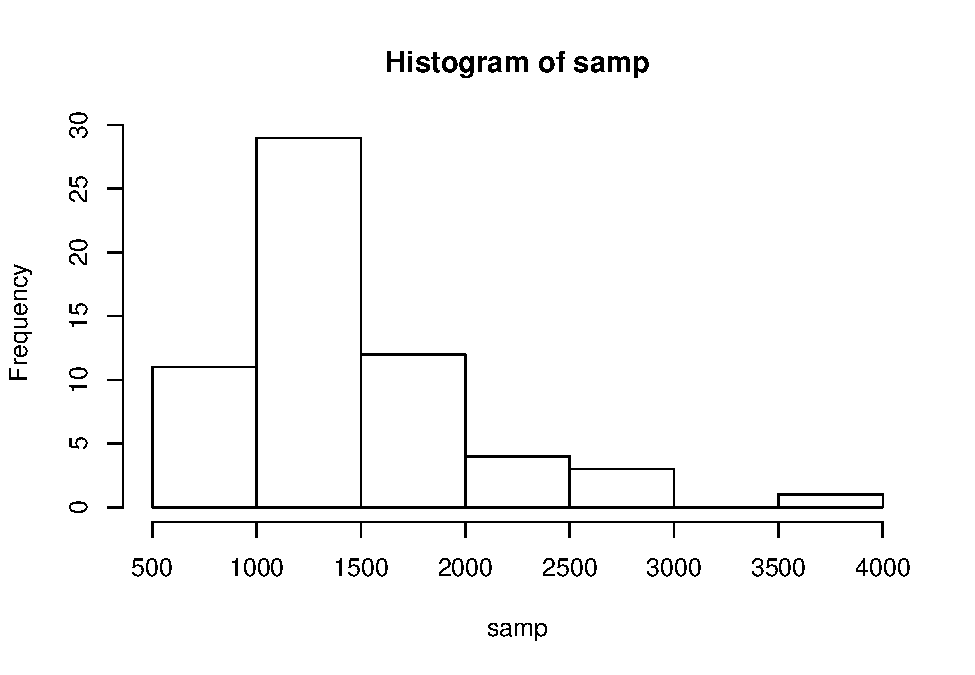
\includegraphics{DATA_606_Lab_4b_files/figure-latex/questone-1.pdf}

The sample's distribution is unimodal, with a right skew. The typical
size would be the most common size, which, in this case, would be near
the mean, which is 1,444.

\subsection{Question 2}\label{question-2}

\begin{enumerate}
\def\labelenumi{\arabic{enumi}.}
\setcounter{enumi}{1}
\tightlist
\item
  Would you expect another student's distribution to be identical to
  yours? Would you expect it to be similar? Why or why not?
\end{enumerate}

\subsubsection{Solution}\label{solution-1}

Since this is a random sample with \(n > 30\), I would expect a similar
but different distribution.

\subsection{Confidence intervals}\label{confidence-intervals}

One of the most common ways to describe the typical or central value of
a distribution is to use the mean. In this case we can calculate the
mean of the sample using,

\begin{Shaded}
\begin{Highlighting}[]
\NormalTok{sample_mean <-}\StringTok{ }\KeywordTok{mean}\NormalTok{(samp)}
\end{Highlighting}
\end{Shaded}

Return for a moment to the question that first motivated this lab: based
on this sample, what can we infer about the population? Based only on
this single sample, the best estimate of the average living area of
houses sold in Ames would be the sample mean, usually denoted as
\(\bar{x}\) (here we're calling it \texttt{sample\_mean}). That serves
as a good \emph{point estimate} but it would be useful to also
communicate how uncertain we are of that estimate. This can be captured
by using a \emph{confidence interval}.

We can calculate a 95\% confidence interval for a sample mean by adding
and subtracting 1.96 standard errors to the point estimate (See Section
4.2.3 if you are unfamiliar with this formula).

\begin{Shaded}
\begin{Highlighting}[]
\NormalTok{se <-}\StringTok{ }\KeywordTok{sd}\NormalTok{(samp) }\OperatorTok{/}\StringTok{ }\KeywordTok{sqrt}\NormalTok{(}\DecValTok{60}\NormalTok{)}
\NormalTok{lower <-}\StringTok{ }\NormalTok{sample_mean }\OperatorTok{-}\StringTok{ }\FloatTok{1.96} \OperatorTok{*}\StringTok{ }\NormalTok{se}
\NormalTok{upper <-}\StringTok{ }\NormalTok{sample_mean }\OperatorTok{+}\StringTok{ }\FloatTok{1.96} \OperatorTok{*}\StringTok{ }\NormalTok{se}
\KeywordTok{c}\NormalTok{(lower, upper)}
\end{Highlighting}
\end{Shaded}

\begin{verbatim}
## [1] 1296.827 1590.506
\end{verbatim}

This is an important inference that we've just made: even though we
don't know what the full population looks like, we're 95\% confident
that the true average size of houses in Ames lies between the values
\emph{lower} and \emph{upper}. There are a few conditions that must be
met for this interval to be valid.

\subsection{Question 3}\label{question-3}

\begin{enumerate}
\def\labelenumi{\arabic{enumi}.}
\setcounter{enumi}{2}
\tightlist
\item
  For the confidence interval to be valid, the sample mean must be
  normally distributed and have standard error \(s / \sqrt{n}\). What
  conditions must be met for this to be true?
\end{enumerate}

\subsubsection{Solution}\label{solution-2}

The sample must be somewhat large (\(n > 30\)), IID (independent:
\(< 10\%\) of the population), and not (strongly) skewed.

\subsection{Confidence levels}\label{confidence-levels}

\subsection{Question 4}\label{question-4}

\begin{enumerate}
\def\labelenumi{\arabic{enumi}.}
\setcounter{enumi}{3}
\tightlist
\item
  What does ``95\% confidence'' mean? If you're not sure, see Section
  4.2.2.
\end{enumerate}

\subsubsection{Solution}\label{solution-3}

We are \(95\%\) confident that the population mean falls within that
interval.

In this case we have the luxury of knowing the true population mean
since we have data on the entire population. This value can be
calculated using the following command:

\begin{Shaded}
\begin{Highlighting}[]
\KeywordTok{mean}\NormalTok{(population)}
\end{Highlighting}
\end{Shaded}

\begin{verbatim}
## [1] 1499.69
\end{verbatim}

\subsection{Question 5}\label{question-5}

\begin{enumerate}
\def\labelenumi{\arabic{enumi}.}
\setcounter{enumi}{4}
\tightlist
\item
  Does your confidence interval capture the true average size of houses
  in Ames? If you are working on this lab in a classroom, does your
  neighbor's interval capture this value?
\end{enumerate}

\subsubsection{Solution}\label{solution-4}

The confidence interval is \((1296.827, 1590.506)\), so the population
mean (\(1499.69\)) is, indeed, in the interval.

\subsection{Question 6}\label{question-6}

\begin{enumerate}
\def\labelenumi{\arabic{enumi}.}
\setcounter{enumi}{5}
\tightlist
\item
  Each student in your class should have gotten a slightly different
  confidence interval. What proportion of those intervals would you
  expect to capture the true population mean? Why? If you are working in
  this lab in a classroom, collect data on the intervals created by
  other students in the class and calculate the proportion of intervals
  that capture the true population mean.
\end{enumerate}

\subsubsection{Solution}\label{solution-5}

With a large enough sample, I'd expect the percentage of intervals that
are correct to converge toward 95\%, since that is the very definition
of 95\% confident.

Using R, we're going to recreate many samples to learn more about how
sample means and confidence intervals vary from one sample to another.
\emph{Loops} come in handy here (If you are unfamiliar with loops,
review the
\href{http://htmlpreview.github.io/?https://github.com/andrewpbray/oiLabs/blob/master/sampling_distributions/sampling_distributions.html}{Sampling
Distribution Lab}).

Here is the rough outline:

\begin{itemize}
\tightlist
\item
  Obtain a random sample.
\item
  Calculate and store the sample's mean and standard deviation.
\item
  Repeat steps (1) and (2) 50 times.
\item
  Use these stored statistics to calculate many confidence intervals.
\end{itemize}

But before we do all of this, we need to first create empty vectors
where we can save the means and standard deviations that will be
calculated from each sample. And while we're at it, let's also store the
desired sample size as \texttt{n}.

\begin{Shaded}
\begin{Highlighting}[]
\NormalTok{samp_mean <-}\StringTok{ }\KeywordTok{rep}\NormalTok{(}\OtherTok{NA}\NormalTok{, }\DecValTok{50}\NormalTok{)}
\NormalTok{samp_sd <-}\StringTok{ }\KeywordTok{rep}\NormalTok{(}\OtherTok{NA}\NormalTok{, }\DecValTok{50}\NormalTok{)}
\NormalTok{n <-}\StringTok{ }\DecValTok{60}
\end{Highlighting}
\end{Shaded}

Now we're ready for the loop where we calculate the means and standard
deviations of 50 random samples.

\begin{Shaded}
\begin{Highlighting}[]
\ControlFlowTok{for}\NormalTok{(i }\ControlFlowTok{in} \DecValTok{1}\OperatorTok{:}\DecValTok{50}\NormalTok{)\{}
\NormalTok{  samp <-}\StringTok{ }\KeywordTok{sample}\NormalTok{(population, n) }\CommentTok{# obtain a sample of size n = 60 from the population}
\NormalTok{  samp_mean[i] <-}\StringTok{ }\KeywordTok{mean}\NormalTok{(samp)    }\CommentTok{# save sample mean in ith element of samp_mean}
\NormalTok{  samp_sd[i] <-}\StringTok{ }\KeywordTok{sd}\NormalTok{(samp)        }\CommentTok{# save sample sd in ith element of samp_sd}
\NormalTok{\}}
\end{Highlighting}
\end{Shaded}

Lastly, we construct the confidence intervals.

\begin{Shaded}
\begin{Highlighting}[]
\NormalTok{lower_vector <-}\StringTok{ }\NormalTok{samp_mean }\OperatorTok{-}\StringTok{ }\FloatTok{1.96} \OperatorTok{*}\StringTok{ }\NormalTok{samp_sd }\OperatorTok{/}\StringTok{ }\KeywordTok{sqrt}\NormalTok{(n) }
\NormalTok{upper_vector <-}\StringTok{ }\NormalTok{samp_mean }\OperatorTok{+}\StringTok{ }\FloatTok{1.96} \OperatorTok{*}\StringTok{ }\NormalTok{samp_sd }\OperatorTok{/}\StringTok{ }\KeywordTok{sqrt}\NormalTok{(n)}
\end{Highlighting}
\end{Shaded}

Lower bounds of these 50 confidence intervals are stored in
\texttt{lower\_vector}, and the upper bounds are in
\texttt{upper\_vector}. Let's view the first interval.

\begin{Shaded}
\begin{Highlighting}[]
\KeywordTok{c}\NormalTok{(lower_vector[}\DecValTok{1}\NormalTok{], upper_vector[}\DecValTok{1}\NormalTok{])}
\end{Highlighting}
\end{Shaded}

\begin{verbatim}
## [1] 1343.284 1562.583
\end{verbatim}

\begin{center}\rule{0.5\linewidth}{\linethickness}\end{center}

\subsection{On your own}\label{on-your-own}

\subsubsection{1}\label{section}

Using the following function (which was downloaded with the data set),
plot all intervals. What proportion of your confidence intervals include
the true population mean? Is this proportion exactly equal to the
confidence level? If not, explain why.

\begin{Shaded}
\begin{Highlighting}[]
\KeywordTok{plot_ci}\NormalTok{(lower_vector, upper_vector, }\KeywordTok{mean}\NormalTok{(population))}
\end{Highlighting}
\end{Shaded}

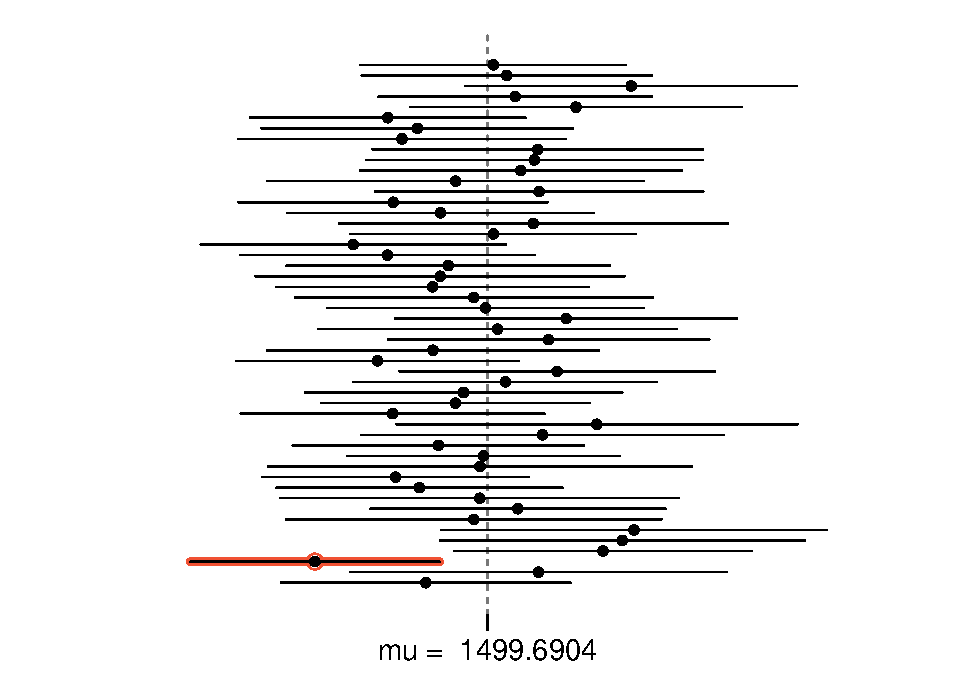
\includegraphics{DATA_606_Lab_4b_files/figure-latex/plot-ci-1.pdf}
\#\#\#\# Solution

\subsubsection{2}\label{section-1}

Pick a confidence level of your choosing, provided it is not 95\%. What
is the appropriate critical value?

\paragraph{Solution}\label{solution-6}

\begin{Shaded}
\begin{Highlighting}[]
\CommentTok{#  For the 98% confidence interval: }
\NormalTok{a <-}\StringTok{ }\DecValTok{1} \OperatorTok{-}\StringTok{ }\FloatTok{0.02}\OperatorTok{/}\DecValTok{2}
\KeywordTok{qnorm}\NormalTok{(a)}
\end{Highlighting}
\end{Shaded}

\begin{verbatim}
## [1] 2.326348
\end{verbatim}

\begin{Shaded}
\begin{Highlighting}[]
\CommentTok{# The critical value is 2.326}
\end{Highlighting}
\end{Shaded}

\subsubsection{3}\label{section-2}

Calculate 50 confidence intervals at the confidence level you chose in
the previous question. You do not need to obtain new samples, simply
calculate new intervals based on the sample means and standard
deviations you have already collected. Using the \texttt{plot\_ci}
function, plot all intervals and calculate the proportion of intervals
that include the true population mean. How does this percentage compare
to the confidence level selected for the intervals?

\paragraph{Solution}\label{solution-7}

\begin{Shaded}
\begin{Highlighting}[]
\NormalTok{lower_vector <-}\StringTok{ }\NormalTok{samp_mean }\OperatorTok{-}\StringTok{ }\FloatTok{2.326} \OperatorTok{*}\StringTok{ }\NormalTok{samp_sd }\OperatorTok{/}\StringTok{ }\KeywordTok{sqrt}\NormalTok{(n) }
\NormalTok{upper_vector <-}\StringTok{ }\NormalTok{samp_mean }\OperatorTok{+}\StringTok{ }\FloatTok{2.326} \OperatorTok{*}\StringTok{ }\NormalTok{samp_sd }\OperatorTok{/}\StringTok{ }\KeywordTok{sqrt}\NormalTok{(n)}
\KeywordTok{plot_ci}\NormalTok{(lower_vector, upper_vector, }\KeywordTok{mean}\NormalTok{(population))}
\end{Highlighting}
\end{Shaded}

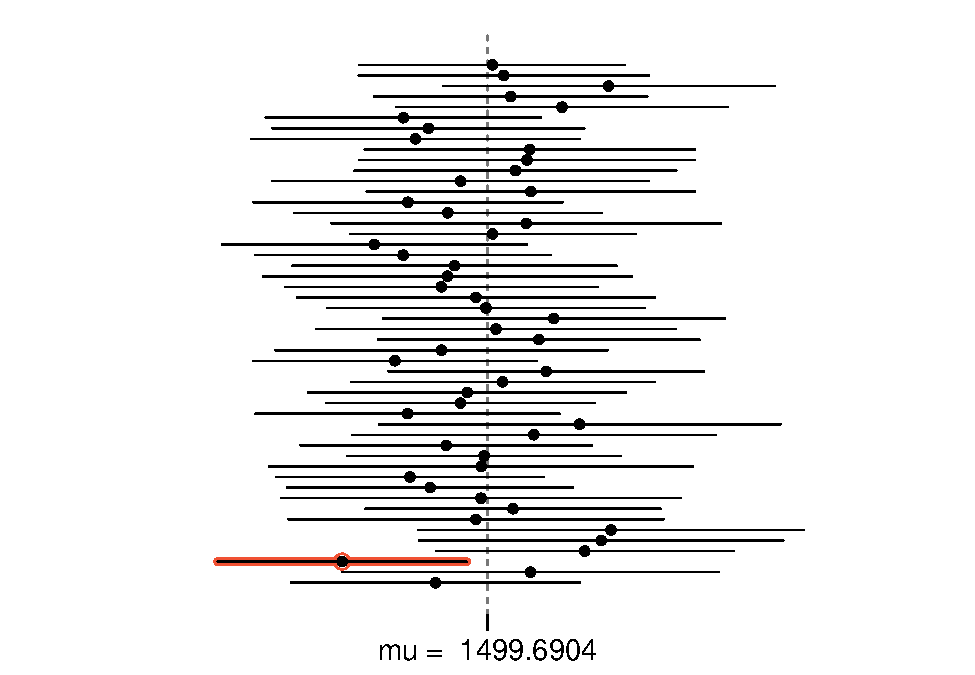
\includegraphics{DATA_606_Lab_4b_files/figure-latex/unnamed-chunk-2-1.pdf}


\end{document}
